\section{Carry Architecture \& Features }

\subsection{Carry Slot Contract}

\subsubsection{Slot Creation}

When a new ad campaign is about to start in a web3 game, the first step is setting up a special ad spot, known as a "slot." This slot is made into a unique digital item, like a one-of-a-kind collectible, which means it's owned and can be traded. Game makers weave these slots into their games, and then either they or the players can activate them, turning them into owned digital assets. It's similar to creating a brand-new collectible item that's ready to be paired with an ad.

\subsubsection{Slot Release}

A slot, once used, may need to be released or made available for future advertisements. This involves the termination or expiration of its current content, making the slot a blank canvas once more. While this could technically be a part of the slot contract, the process's simplicity might not necessitate a full-fledged contract on its own. Instead, it could be an operation under the broader slot management system.


\subsubsection{Slot Content Change}

Over time, advertisements or the content within a slot might need updating or altering. This could be due to changing marketing strategies, game narratives, or even player preferences. The Carry Slot Contract allows for dynamic content modifications, ensuring that the slot remains relevant and engaging.

\subsubsection{Slot Advertisement Placement}

The ultimate purpose of a slot is to showcase advertisements, a process termed 'placement' within the Carry Protocol. It's where the rubber meets the road. Once an advertisement is place into a slot, the slot illuminates, fulfilling its purpose. Placement could involve various parameters like the duration of the advertisement, its visual aesthetics, and interactivity levels, all governed and managed by the Carry Slot Contract.

In essence, the Carry Slot Contract is the backbone of the slot system within the Carry Protocol. It ensures that every slot's lifecycle, from creation to placement, is managed efficiently, transparently, and in harmony with the game's environment and the players' expectations.


\subsection{Carry Measurement \& Metrics}

In the dynamic realm of web3 gaming, the Carry Protocol recognizes the value of real-time feedback for in-game advertising. Through Performance Benchmark Metrics, the protocol offers immediate insights into the impact and success of each advertising slot. Carry analysis features can be described by Figure \ref{fig:analysis}.

These metrics don't just offer a retrospective view, they enable active experimentation within games. By analyzing slot performance, developers can refine ad placements, content, and interactivity. This isn't just about placing an ad—it's about optimizing its reach and engagement in a gaming environment.

Additionally, these metrics provide a twofold benefit:

\begin{itemize}
    \item \textbf{For Game Developers:} They get a clear understanding of how integrated advertisements impact gameplay. This ensures that the core gaming experience remains uncompromised while still being monetizable.
    \item \textbf{For Advertisers:} With concrete performance data, advertisers can refine their campaigns. They can tailor content based on which slots garner the most attention, where players spend the most time, and which in-game scenarios drive the most engagement.
\end{itemize}

\begin{figure}[!htb]
    \centering
    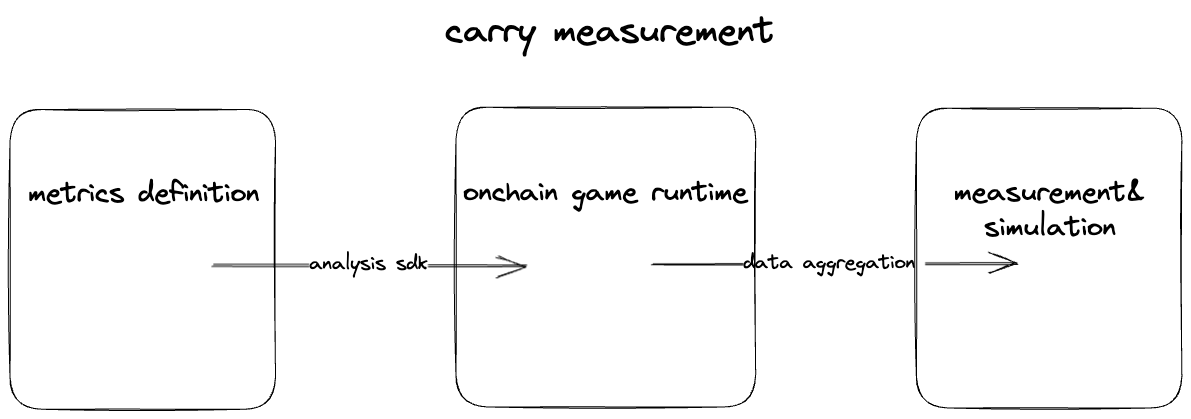
\includegraphics[width=0.8\textwidth]{Figures/measurement.png}
    \caption{Carry Analysis Structure}
    \label{fig:analysis}
\end{figure}


\subsubsection{Experimentation}


The Carry Protocol includes a special feature that lets you try out different strategies directly within the blockchain system to see what works best. This tool uses smart contracts, which are like automated rules, to make a secure space for testing. Here, you can change settings and watch how they affect outcomes, helping you make better decisions as you go along.

Core concepts in experimentation for Carry are:

\textbf{Variables:} A variable is the basic unit which strategy makers are trying to measure. Whether it's the slot's visibility, its position in the gaming interface, or the duration of the ad it holds, these variables dictate the behavior of users, regarding certain types of slots. Adjusting them using decentralized logic helps to find the optimal setting for each slot or group of slots.

\textbf{Groups:} Groups can be a collection of any basic unit in the entire carry protocol, cluster of slots, chosen user addresses, gamers in a certain region etc. Groups are a tool for conducting experiments in a scalable way.

\textbf{Experiments:} Each 'experiment' revolves around these slots and their groups. Being smart contracts, they execute tests autonomously on these slot configurations. The experiments can range from testing a new slot position to trying out different ad durations. As these experiments run, they yield data, offering insights into the most effective slot configurations.

\textbf{Rollouts:} Once an experiment concludes, the 'rollouts' come into play. They are the action-driven aftermath of successful experiments, ensuring that proven slot configurations, those variables and group settings that worked, are implemented across the board. It's like upgrading a group of slots based on real, tested data.

In conclusion, experimentation will greatly help users to measure the performance of their strategies. By enabling experimentation, they ensure that the convergence of gaming and advertising is not just seamless but also continually evolving, adaptive, and player-centric.

\subsubsection{Metrics}

Metrics in the Carry Protocol stand as instrumental indicators, vital in understanding the nuances of in-game advertising in the vast expanse of web3 gaming. Serving as both compass and map, these metrics provide developers and advertisers with real-time insights into the effectiveness and resonance of each ad slot. Notably, these metrics encompass:

\begin{itemize}
    \item \textbf{Actual Views}: Capturing the raw count of users who engage with an ad.
    \item \textbf{Viewer Profiles}: A snapshot of user demographics, interests, and behaviors, allowing for targeted advertising.
    \item \textbf{Conversion Metrics}: Indicators that show the transition of viewers from mere observers to engaged participants or customers.
    \item \textbf{On-chain Payments}: Metrics that display the number of transactions linked to a particular advertisement or slot.
    \item \textbf{Staking Participation}: Data on users who are not just viewing ads but actively staking their tokens or assets.
    \item \textbf{Activation Data}: Metrics highlighting the active engagement and interaction of users with an advertisement.
    \item \textbf{App Installation Data}: Monitoring the number of users who, upon viewing an ad, proceed to install the promoted app.
    \item \textbf{Community Engagement}: Data on users redirected to and actively participating in the advertised community forums or platforms.
    \item \textbf{Social Media Engagement}: Monitoring the traction on social media platforms due to the advertisement, gauging the viral potential of ads.
\end{itemize}

With these metrics at their fingertips, users can refine their advertisement strategies. They ensure that the ad content doesn't merely inhabit a slot but actively engages, informs, and captivates the gaming audience, optimizing both visibility and impact.




